

\subsection{Photodiode}
\label{sec:photodiode}

\todo[inline]{amplifier not rail to rail, write that}

The photodiode is used to detect the intensity of the light shined upon it.
In operation it generates a current proportional to the intensity of the surrounding light.
This signal does, however, need to be converted into a voltage between 0 and 3.3V for the ADC to measure.

To do this, the signal is amplified using the amplifier circuit shown in figure \ref{fig:photodiodeschematics}.
The amplification was found by dimensioning the resistor such that it is close to saturation when the photodiode is exposed to the highest expected lighting level.


\begin{figure}[H]
\centering 
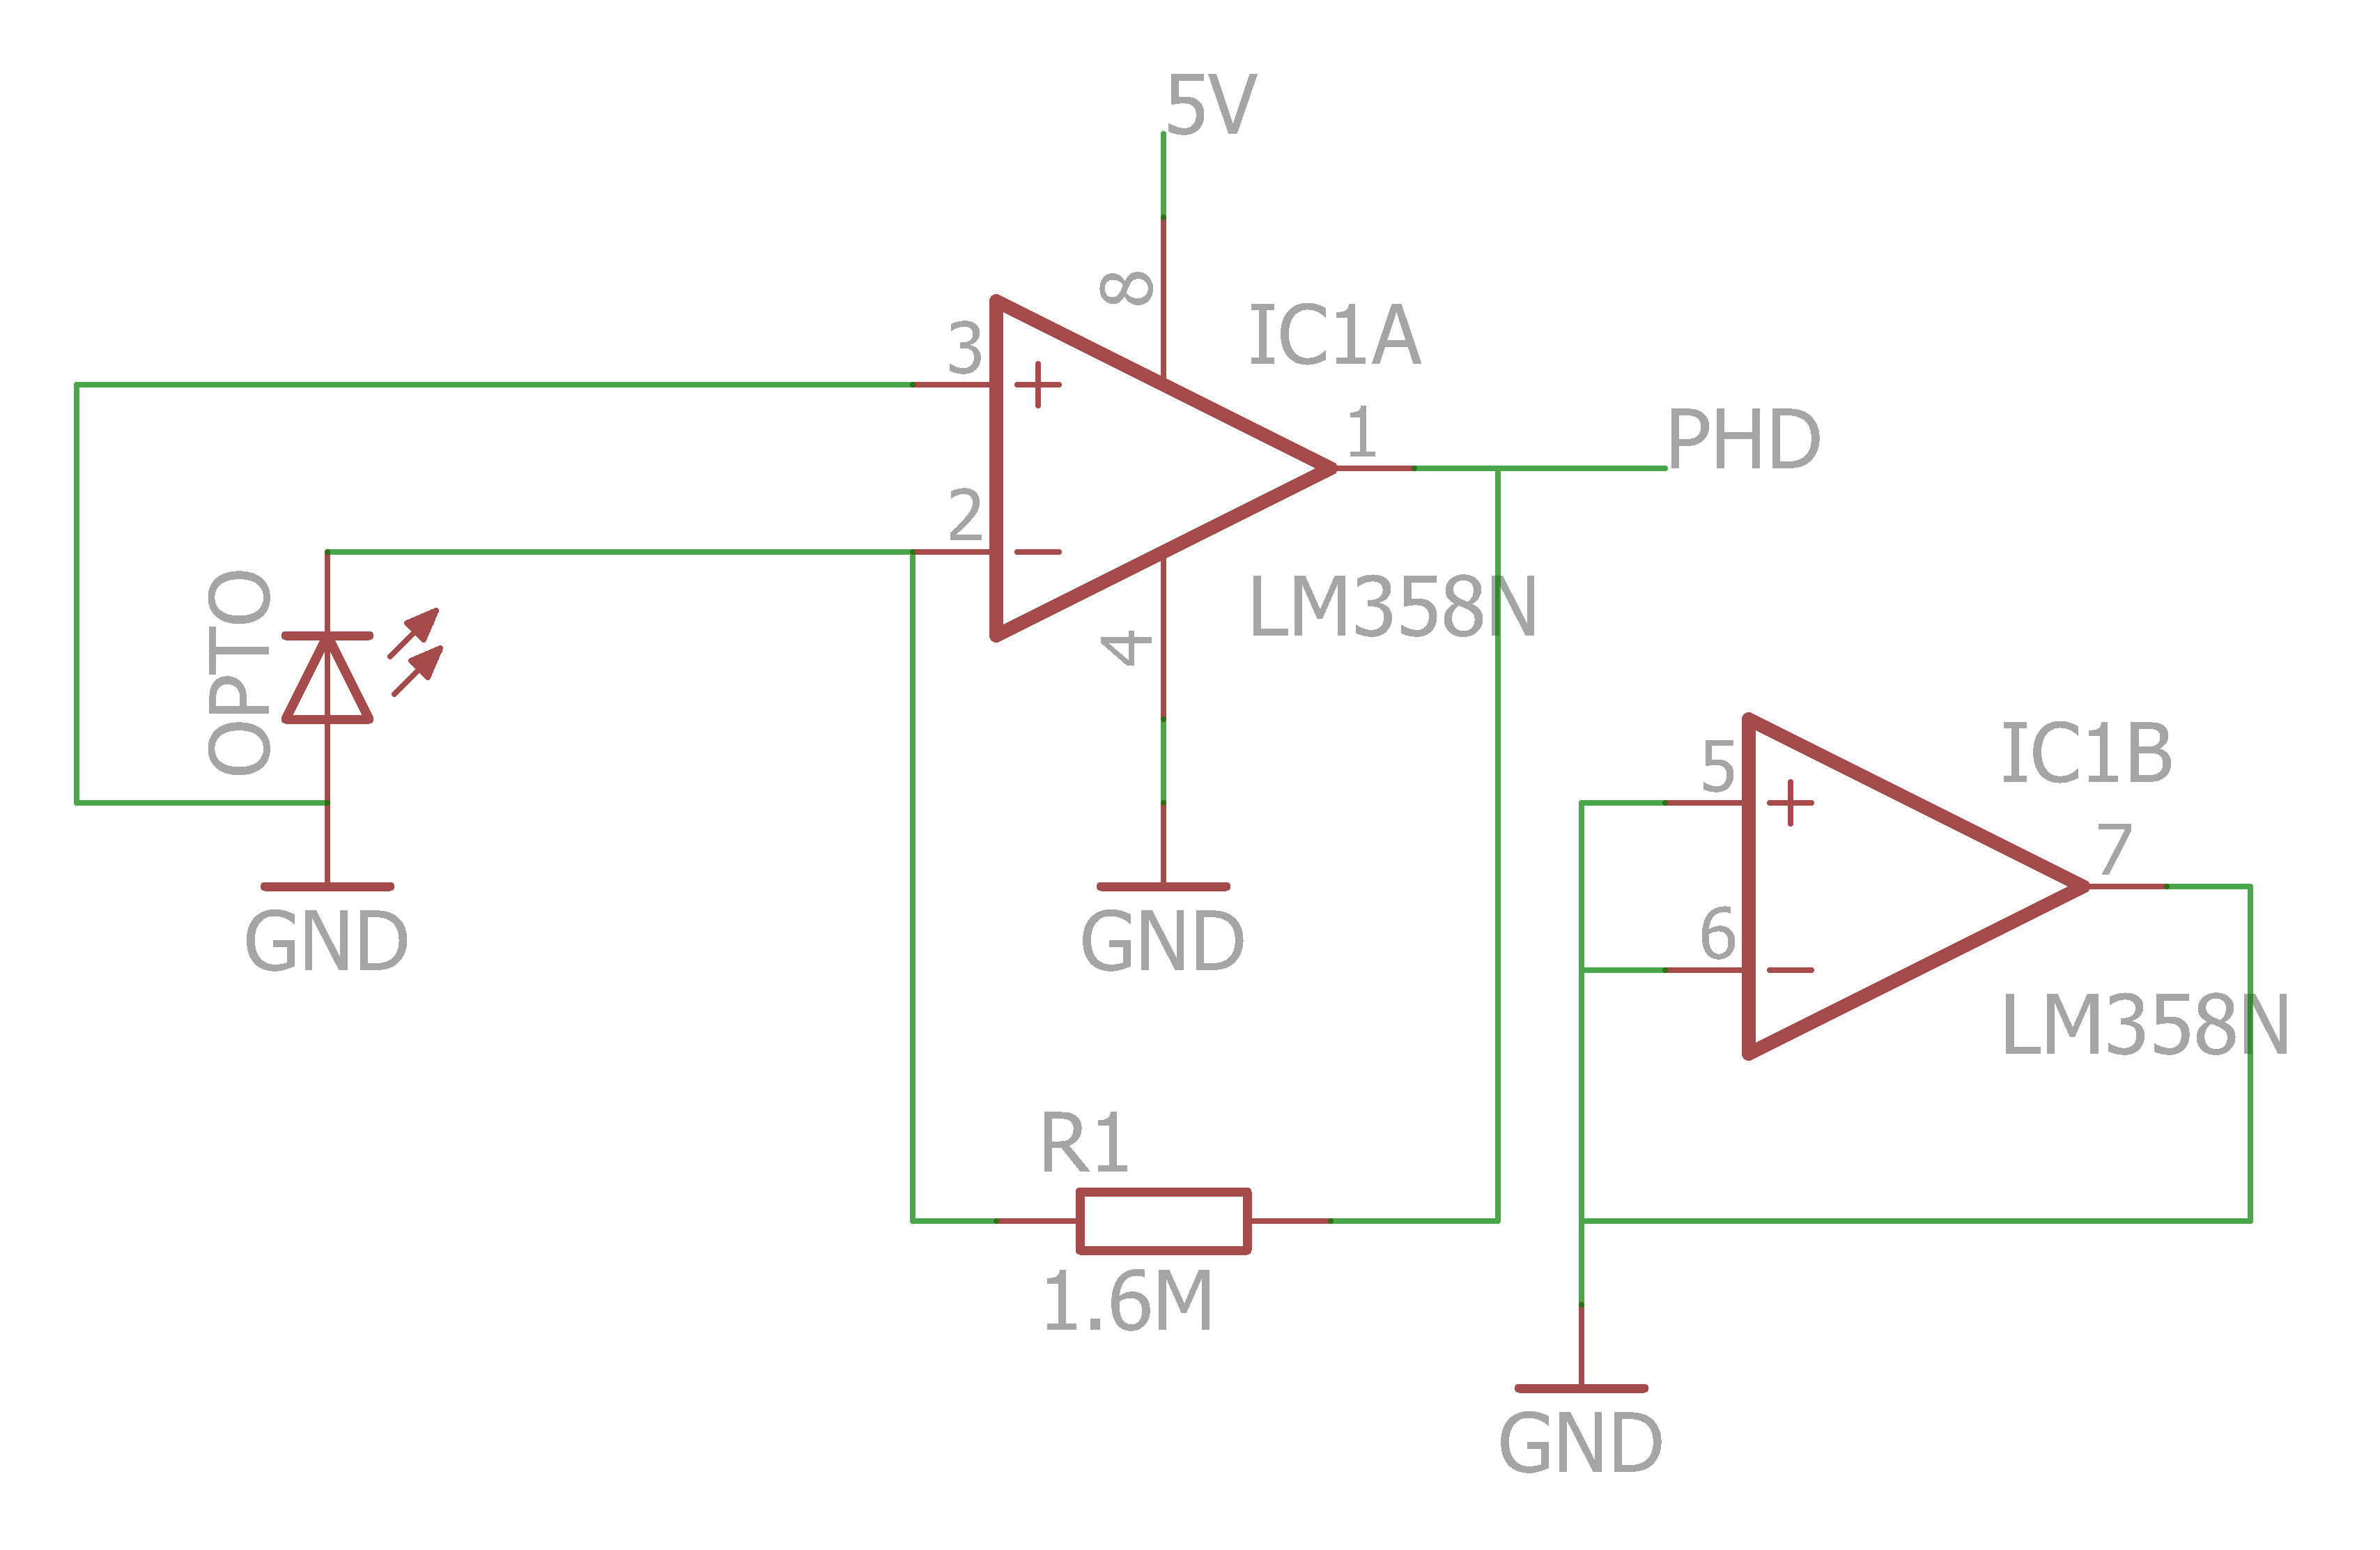
\includegraphics[width = 0.6 \textwidth]{images/optoamplifier_schematics}
\caption{Photodiode amplifier schematics.}
\label{fig:photodiodeschematics}
\end{figure}

As seen in figure \ref{fig:photodiodeschematics} a LM358N \footnote{\href{http://docs-europe.electrocomponents.com/webdocs/0780/0900766b807800ef.pdf}{LM358N Datasheet}} was chosen as the operational amplifier.
This amplifier was chosen because it is  a general purpose amplifier and no other specific requirements were needed.

The second amplifier in the package is circuited completely to ground, as seen on figure \ref{fig:photodiodeschematics}, since it is not in use.

The output of the amplifier (PHD, in figure \ref{fig:photodiodeschematics}) is then routed directly to the ADC port (OPTO, in figure \ref{fig:adc_schematics}).
The ADC used is the MCP3008\footnote{ \url{https://www.adafruit.com/datasheets/MCP3008.pdf} }.


\begin{figure}[H]
\centering 
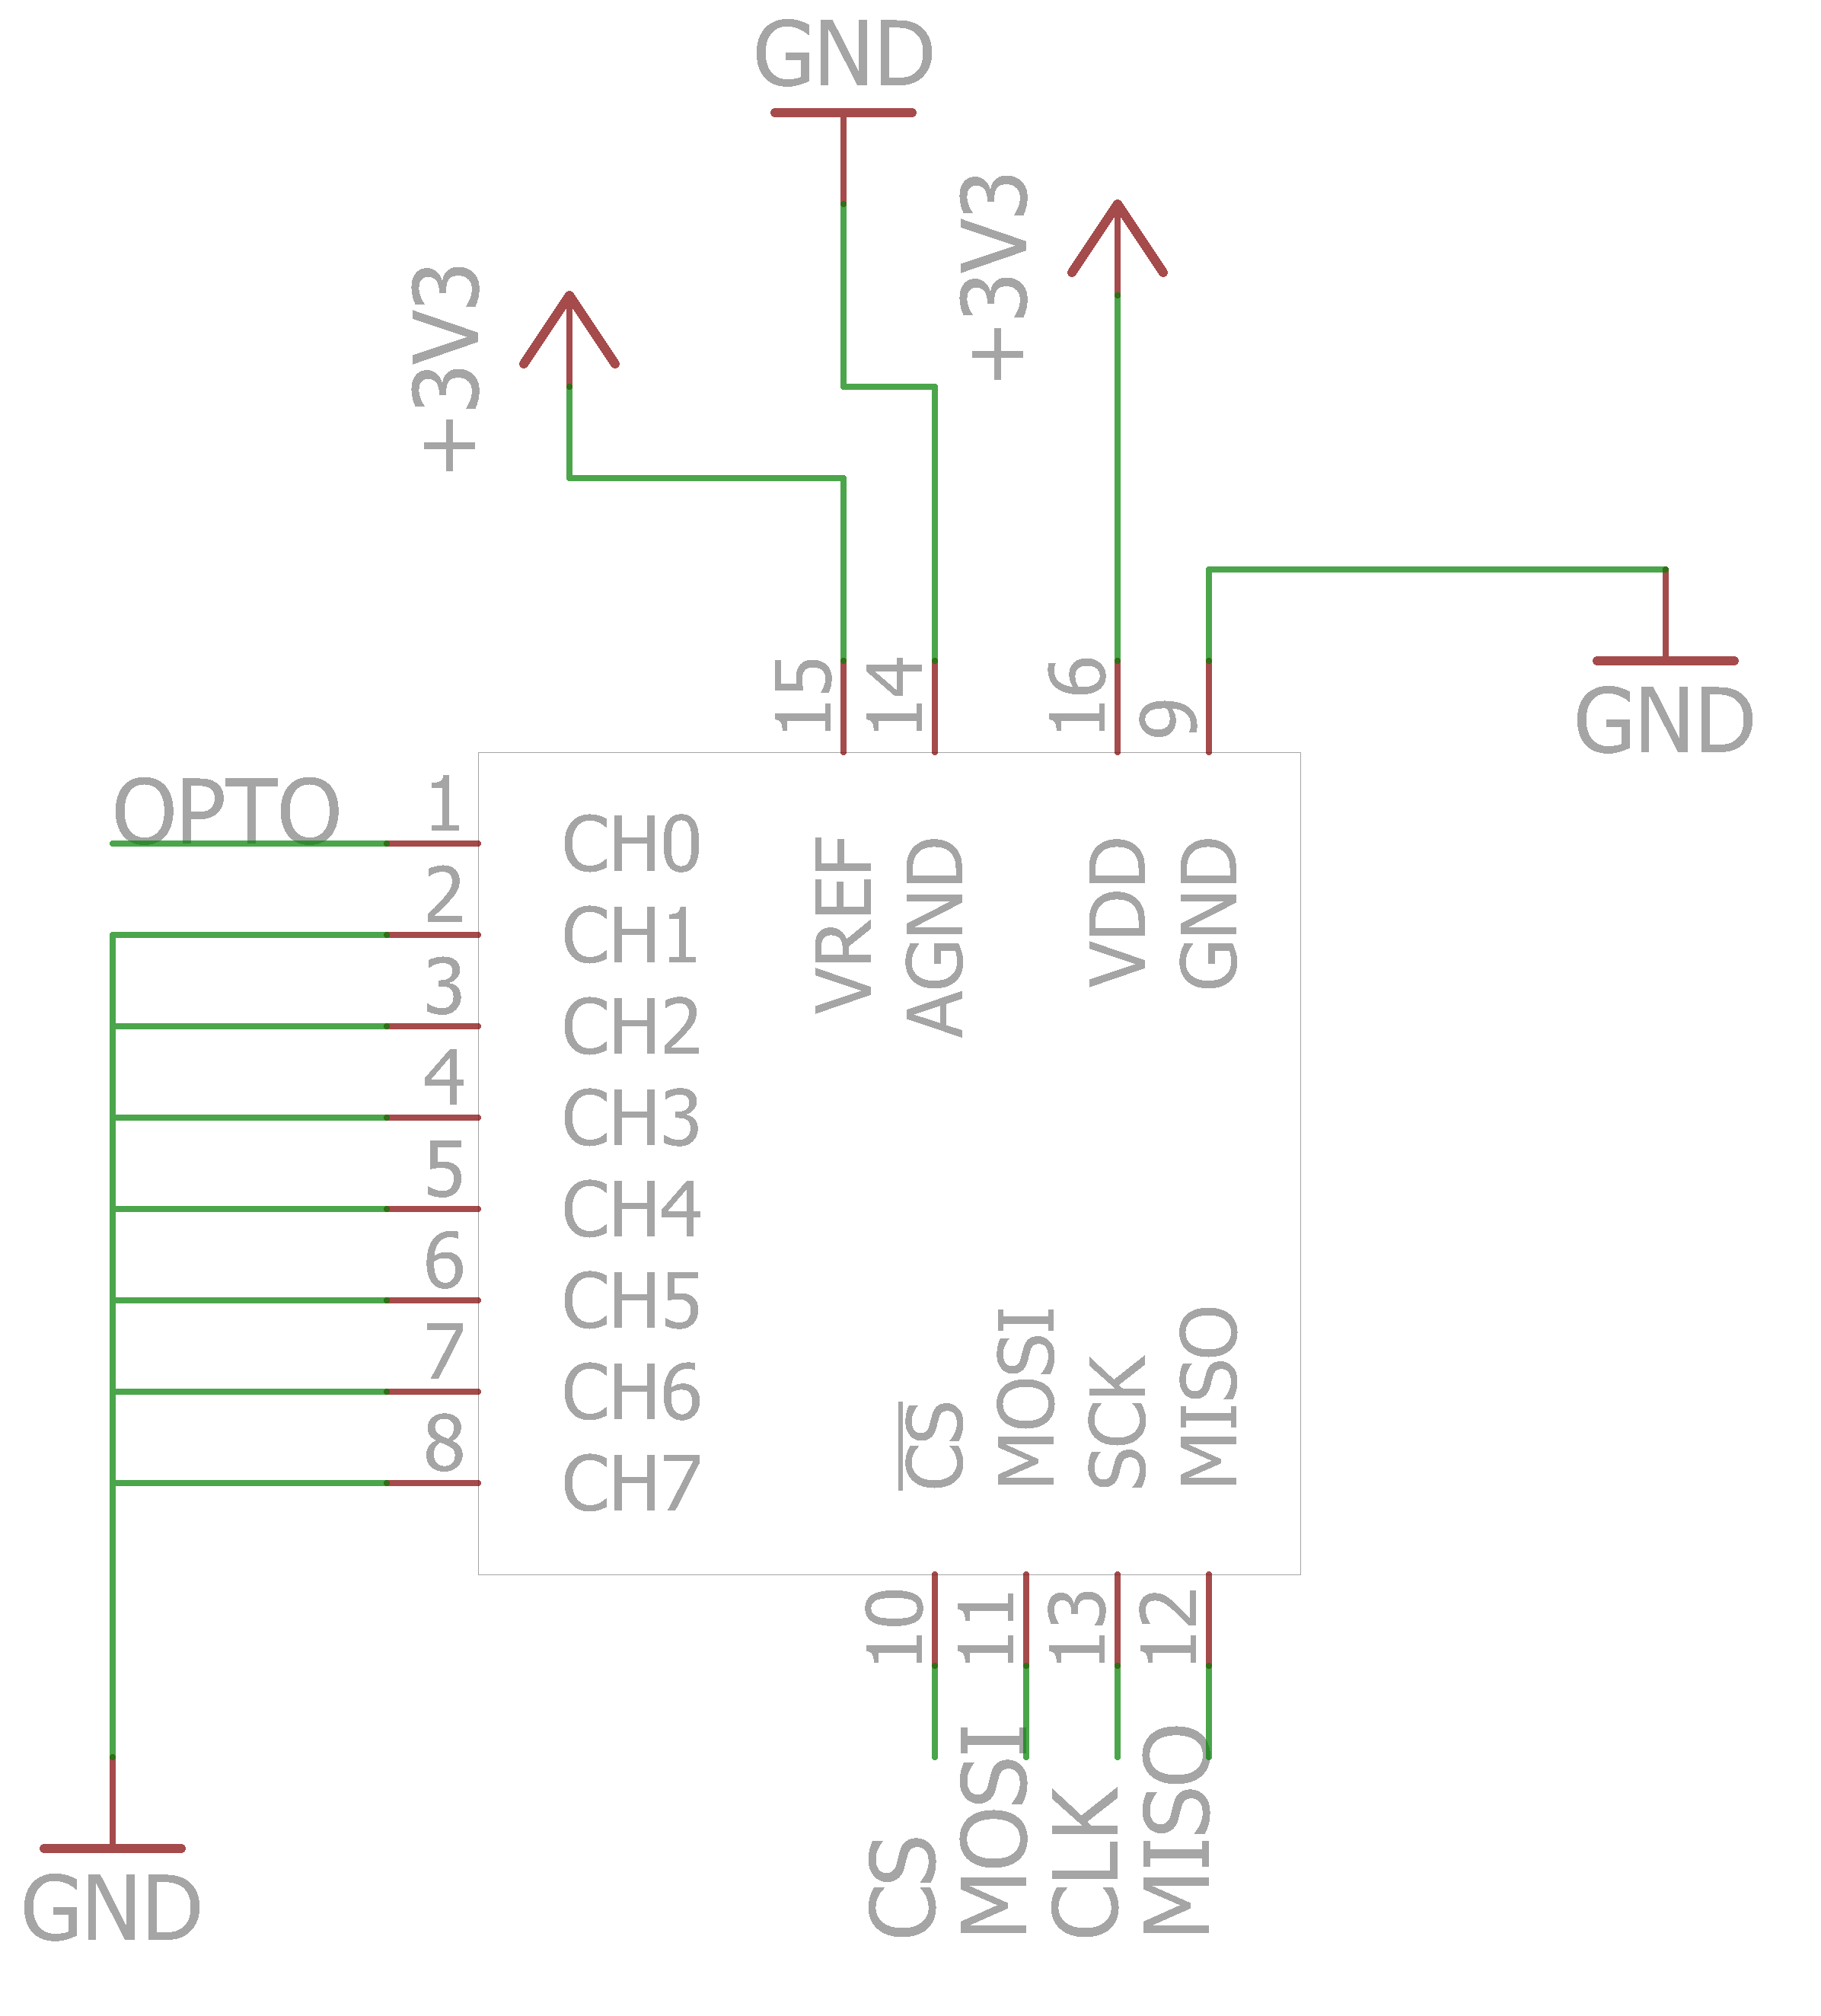
\includegraphics[width = 0.4 \textwidth]{images/ADC_schematics}
\caption{Schematics of the ADC connections.}
\label{fig:adc_schematics}
\end{figure}


To test the final signal of the photodiode circuit the output of amplifier was compared to the output of the LEDs when these are turned on and off one after the other.
The result of such is seen in figure \ref{fig:photodiode_output}.
It can be seen on figure \ref{fig:photodiode_output} that when the LED's switch color, this results in oscillations about the resulting voltage.
When sampled at this time the data would hence be wrong.
This problem can be solved by adding a low-pass filter to the amplifier circuit to reduce/remove the oscillations or one could wait with sampling the signal until it has stabilized.
Of these two options the latter was used.
This was chosen because the number of samples gathered a second, even when not being able to sample directly after the LED has turned on, is still so high that the sample frequency is a problem.
The sample for each color is hence first taken $3.3 \cdot 10^-5 s$ after the LED is turned on.


\begin{figure}[H]
\centering 
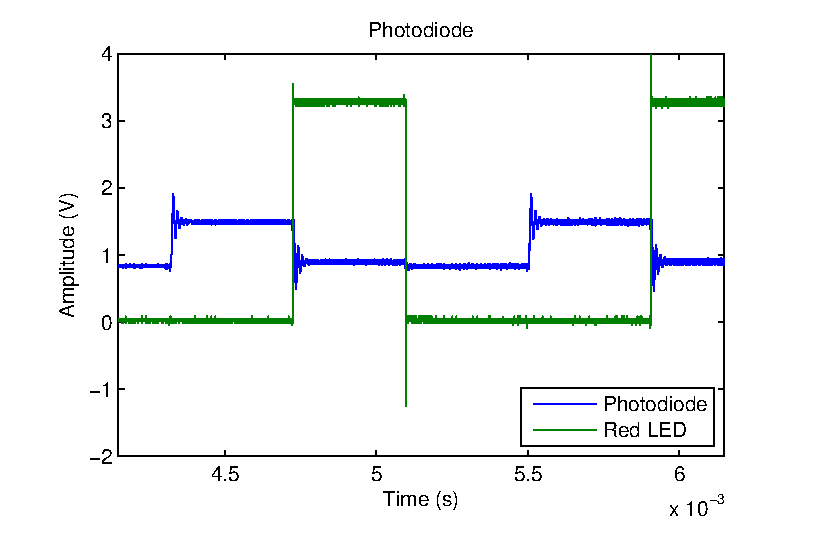
\includegraphics[width = 0.9 \textwidth]{images/photodiode}
\caption{Output of the photodiode amplification versus the signal to the red LED.}
\label{fig:photodiode_output}
\end{figure}

It is also noticeable that the amplifier is not a rail-to-rail amplifier and the input to the ADC can hence not reach the 3.3V before it reaches saturation.
This reduce the resolution of the light-intensity measurable by the system.
This problem could be solved by supplying the amplifier with a higher voltage such that its saturation is at 3.3V, or higher, or one could use a rail-to-rail amplifier, which can be more expensive.
This problem was, however, not deemed necessary for the project as the resolution of the light intensity still is high enough to detect the difference among the different brick colors.




